\subsection{Model-Based Safety Assessment Process Supported by Formal Methods}
\label{subsec:process}
We propose a model-based safety assessment process backed by formal methods to help safety engineers with early detection of design issues.  This process uses a single unified model to support both system design and safety analysis. It is based on the following steps as shown in Figure~\ref{fig:updated_safety_process} and outlined below.

\begin{figure}[t!]
	
	\centering
	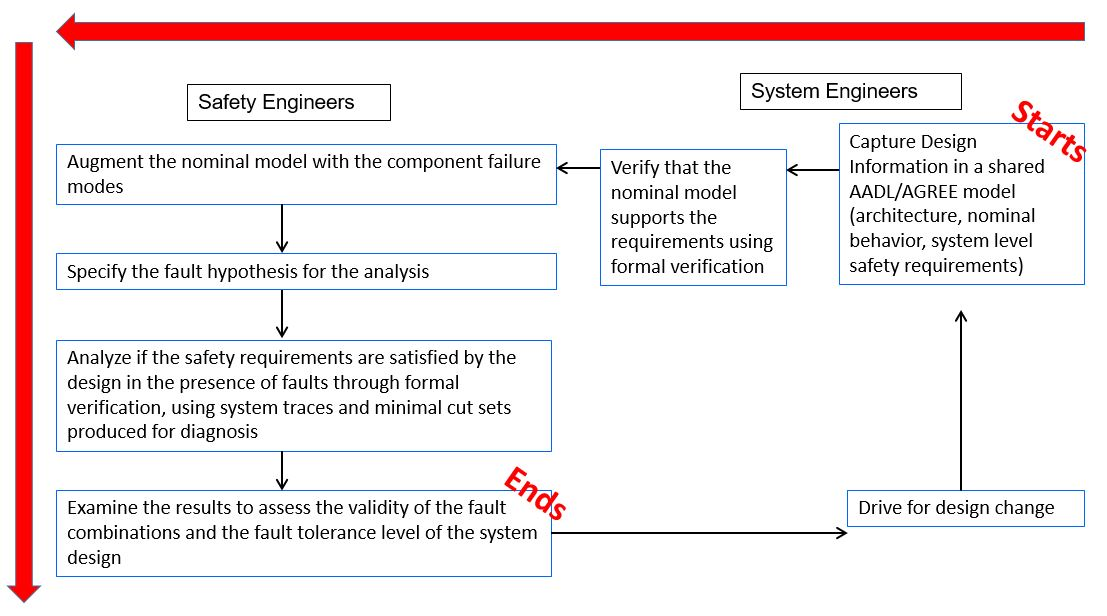
\includegraphics[width=0.85\textwidth]{images/process4.jpg}
	
	\caption{Proposed Safety Assessment Process Backed by Formal Methods}
	\label{fig:updated_safety_process}
\end{figure}

\begin{enumerate}
	\item System engineers capture the critical information in a shared \gls{aadl}/\gls{agree} model:  high-level hardware and software architecture, nominal behavior at the component level, and safety requirements at the system level.% (e.g., inhibit throttle movement during critical takeoff phase).
	\item System engineers use the backend model checker to verify that the nominal model supports the requirements.
	\item Safety engineers use the Safety Annex to augment the nominal model with the component failure modes. % (e.g., processor failure, input signal corrupted).  
	In addition, safety engineers specify the fault hypothesis for the analysis which corresponds to how many simultaneous faults the system must be able to tolerate.
	\item Safety engineers use the backend model checker to analyze if the safety requirements and fault tolerance objectives are satisfied by the model in the presence of faults. % (e.g., if the system is resilient to a single failure). 
	If the model design does not tolerate the specified number of faults (or probability threshold of fault occurrence), then the tool produces counterexamples leading to safety requirement violation in the presence of faults, %and also
	 as well as all minimal sets of fault combinations that can cause the safety requirement to be violated.
	%produces fault trees showing smallest set of faults that may lead to the safety requirement being violated. 
	\item The safety engineers examine the results to assess the validity of the fault combinations and the fault tolerance level of the system design. If a design change is warranted, the model will be updated with the latest design change and the above process is repeated.
\end{enumerate}

There are other tools purpose-built for safety analysis, including AltaRica~\cite{PROSVIRNOVA2013127}, smartIFlow~\cite{info17:HaLuHo} and xSAP~\cite{DBLP:conf/tacas/BittnerBCCGGMMZ16}. These tools and their accompanying notations are separate from the system development model. Other tools extend existing system models, such as HiP-HOPS~\cite{CHEN201391} and the \gls{aadl} Error Model Annex, Version 2 (EMV2)~\cite{EMV2}. EMV2 uses enumeration of faults in each component and explicit propagation of faulty behavior to perform error analysis. The required propagation relationships must be manually added to the system model and can become complex, leading to mistakes in the analysis.

In contrast, the Safety Annex supports model checking and quantitative reasoning by attaching behavioral faults to components and then using the normal behavioral propagation and proof mechanisms built into the \gls{agree} \gls{aadl} annex.  This allows users to reason about the evolution of faults over time, and produce counterexamples demonstrating how component faults lead to failures.
Our approach extends and adapts the work of Joshi et al.~\cite{Joshi05:Dasc} to the \gls{aadl} modeling language.  
%Stewart, et. al provide more information on the approach~\cite{Stewart17:IMBSA}, and 
The tool and documentation are made available under a BSD license and can be located at: \small \url{https://github.com/loonwerks/AMASE/}. \normalsize